% Provenance (never printed): NSI premiere "Architectures materielles et systemes d'exploitation" (modele de von
% Neumann, langage machine, assembleur), NSI terminale "systemes sur puce". See sources/book2/BRIEFS.md.
\chapter{The von Neumann Machine and Assembly Language}\label{ch:g11:von-neumann-machine}

In a computer's memory, the instruction ``add register $2$ to register $1$'' and the number $17$ followed by the
number $2$ are the same two bytes. The processor cannot tell them apart; it reads whatever its program counter
points at, and runs it as an instruction. This single idea, program and data in the same memory, is what makes a
computer able to load a new program as easily as new data, and it is also why a wrong write can turn data into
code.

This chapter takes the toy machine of Book 1 seriously: its whole \omterm{def:g11:von-neumann-machine:instruction-set}{instruction set}, programs with \omterm{def:g11:von-neumann-machine:jump}{jumps} and loops, the
stack and \omterm{def:g11:von-neumann-machine:subroutine}{subroutines}, and the step from a line of Python down to the machine's instructions.

\begin{recall}
A processor repeats the same cycle: fetch the instruction at the address in the program counter, decode it, execute
it. Its registers are a few fast cells inside it; machine language is the numbers that encode its instructions; a
chip may hold several cores, each running its own program (Book 1, grade 7). An adder, a \omterm{def:g11:gates-to-arithmetic-unit:mux}{multiplexer} and a register of
\omterm{def:g11:gates-to-arithmetic-unit:latch}{flip-flops} are built from gates (the previous chapter).
\end{recall}

\section{Processor, memory, buses}\label{sec:g11:von-neumann-machine:model}

\begin{definition}[von Neumann architecture]\label{def:g11:von-neumann-machine:von-neumann}
A computer has a \emph{von Neumann architecture}\index{von Neumann architecture} when it is made of a processor (a
control unit, an ALU and registers), one memory that holds both the program and its data, and input and output
devices, and when the processor runs the program by fetching its instructions from that memory one after the other.
\end{definition}

\begin{definition}[Bus]\label{def:g11:von-neumann-machine:bus}
A \emph{bus}\index{bus} is a set of wires shared by several components to carry one kind of signal. The
\emph{address bus} carries the number of the memory cell or device being accessed, the \emph{data bus} the value
read or written, and the \emph{control bus} the signals that say what to do and when, such as ``read'' or ``write''.
\end{definition}

\begin{omfigure}
\begin{tikzpicture}[font=\small, box/.style={draw, rounded corners=2pt, align=center, inner sep=4pt}]
  \node[box, fill=omDef!8, minimum width=46mm, minimum height=30mm] (cpu) at (0,0) {};
  \node[font=\bfseries\small, anchor=north] at (cpu.north) {processor};
  \node[box, fill=white, minimum width=18mm] (cu) at (-1.15,0.15) {control\\unit};
  \node[box, fill=white, minimum width=14mm] (alu) at (1.2,0.15) {ALU};
  \node[box, fill=white, minimum width=40mm, font=\footnotesize] (reg) at (0,-0.95) {registers, PC, SP, flags};
  \node[box, fill=omMeth!10, minimum width=26mm, minimum height=30mm] (mem) at (4.3,0) {memory\\[2pt]program\\and data};
  \node[box, fill=omProp!10, minimum width=24mm, minimum height=30mm] (io) at (7.3,0) {input\\and\\output};
  \foreach \y/\n/\c in {-2.4/address bus/omThm, -2.9/data bus/omDef, -3.4/control bus/omMeth} {
    \draw[very thick, \c] (-2.3,\y) -- (8.7,\y);
    \node[anchor=west, font=\footnotesize, text=\c] at (8.8,\y) {\n};
  }
  \foreach \x in {0, 4.3, 7.3} {
    \draw[thick, omThm] (\x-0.7,-1.5) -- (\x-0.7,-2.4);
    \draw[thick, omDef] (\x,-1.5) -- (\x,-2.9);
    \draw[thick, omMeth] (\x+0.7,-1.5) -- (\x+0.7,-3.4);
  }
\end{tikzpicture}

{\small The von Neumann model. The processor reaches the memory and the devices through the same three buses; one
memory holds the program and its data.}
\end{omfigure}

Each fetch, each \code{LOAD} and each \code{STORE} is a trip over the buses: the processor puts an address on the
address \omterm{def:g11:von-neumann-machine:bus}{bus} and ``read'' on the control \omterm{def:g11:von-neumann-machine:bus}{bus}, and the memory answers on the data \omterm{def:g11:von-neumann-machine:bus}{bus}. A machine with several
processors, or several cores, has them share the memory in the same way, each running its own instructions.

\begin{history}[A report and a baby]
In 1945, the mathematician John von Neumann circulated a \emph{First Draft of a Report on the EDVAC}, which described
a computer keeping its program in the same electronic memory as its data, instead of on plugboards or punched tape.
% ledger: g11:edvac-1945
The first machine to run such a stored program was built in Manchester, England, by Freddie Williams, Tom
Kilburn and Geoff Tootill: nicknamed the Baby, it ran its first program, $17$ instructions written by Kilburn to find
the largest factor of a number, on 21 June 1948.
% ledger: g11:baby-1948
\end{history}

\begin{omfigure}
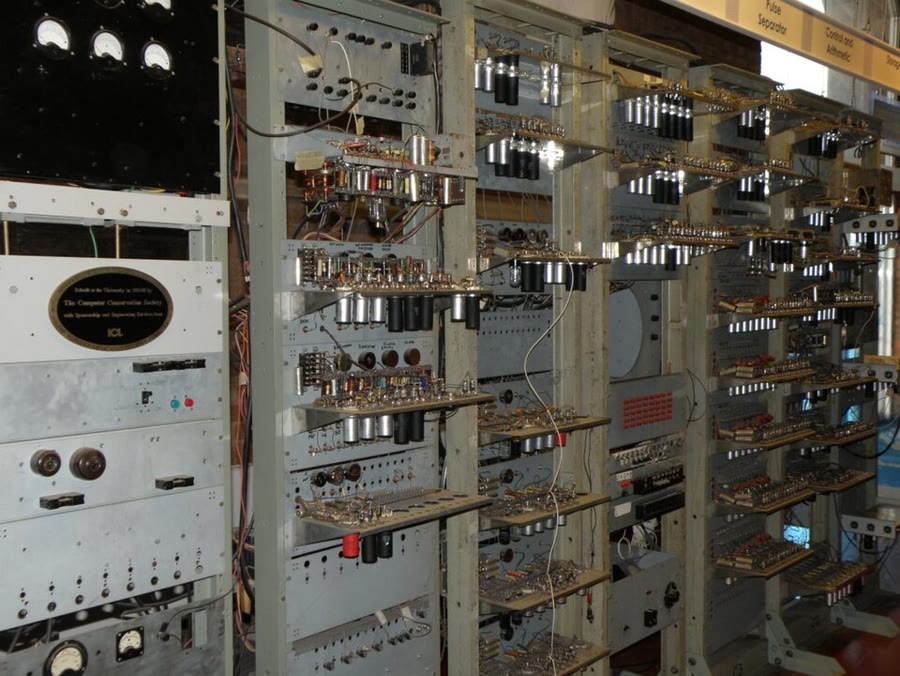
\includegraphics[width=0.55\linewidth]{images/book2/g11-baby-replica.jpg}

{\small A replica of the Baby on display in Manchester: racks of valves, and in the middle the small screen that
showed its memory. Photograph: KGGucwa, CC BY-SA 3.0.}
\end{omfigure}

\section{The toy machine in full}\label{sec:g11:von-neumann-machine:toy}

Book 1 traced small programs of the toy machine by hand. Its full description is short: $256$ cells of one byte, four
registers \code{R0} to \code{R3}, a program counter \code{PC}, a \omterm{def:g11:von-neumann-machine:subroutine}{stack pointer} \code{SP}, and the three flags of the
previous chapter. Arithmetic wraps modulo $256$.

\begin{definition}[Instruction set]\label{def:g11:von-neumann-machine:instruction-set}
The \emph{instruction set}\index{instruction set} of a processor is the list of the instructions it can execute, with
their encoding in bytes and their exact effect on registers, flags and memory.
\end{definition}

The toy machine has $28$ instructions. Each takes two bytes: the first holds a $6$-bit operation code and a $2$-bit
register number, the second an operand: a number, an address, or a second register.

\medskip
\begin{center}
\small
\begin{tabular}{@{}rl@{\qquad}rl@{\qquad}rl@{}}
\hline
0 & \code{HALT} & 10 & \code{NOT r} & 20 & \code{OUT r} \\
1 & \code{LOADI r, n} & 11 & \code{SHL r} & 21 & \code{LOADR r, s} \\
2 & \code{LOAD r, [a]} & 12 & \code{SHR r} & 22 & \code{STORER r, s} \\
3 & \code{STORE r, [a]} & 13 & \code{CMP r, s} & 23 & \code{PUSH r} \\
4 & \code{ADD r, s} & 14 & \code{JMP a} & 24 & \code{POP r} \\
5 & \code{SUB r, s} & 15 & \code{JZ a} & 25 & \code{CALL a} \\
6 & \code{ADDI r, n} & 16 & \code{JNZ a} & 26 & \code{RET} \\
7 & \code{AND r, s} & 17 & \code{JN a} & 27 & \code{NOP} \\
8 & \code{OR r, s} & 18 & \code{JC a} & & \\
9 & \code{XOR r, s} & 19 & \code{IN r} & & \\
\hline
\end{tabular}
\end{center}
\medskip

\noindent \code{LOADI} puts a number in a register, \code{LOAD} and \code{STORE} move a byte between a register and a
cell, and \code{LOADR} and \code{STORER} do the same with the address in a register. The arithmetic and logic
instructions, and \code{CMP}, which subtracts without keeping the result, set the flags $Z$, $N$ and $C$.

\begin{omfigure}
\begin{bytefield}[bitwidth=1.9em]{16}
  \bitheader[endianness=big]{0-15} \\
  \bitbox{6}{operation code} & \bitbox{2}{\code{r}} & \bitbox{8}{operand: \code{n}, \code{a} or \code{s}} \\
  \bitbox{6}{\code{000100} = 4} & \bitbox{2}{\code{01}} & \bitbox{8}{\code{00000010} = 2}
\end{bytefield}

{\small The encoding of an instruction: the first byte is $4 \times \text{operation code} + r$. Below,
\code{ADD R1, R2}: the bytes $4 \times 4 + 1 = 17$ and $2$.}
\end{omfigure}

The step of the machine refines the cycle of Book 1: fetch the two bytes at \code{PC} and \code{PC + 1}, add $2$ to
\code{PC}, decode, execute. A \omterm{def:g11:von-neumann-machine:jump}{jump} writes a new address into \code{PC} after that increment, so the next fetch
happens there.

\section{Assembly programs with jumps}\label{sec:g11:von-neumann-machine:assembly}

\begin{definition}[Assembly language, assembler, label]\label{def:g11:von-neumann-machine:assembly}
An \emph{assembly language}\index{assembly language} writes a machine's instructions with names instead of numbers,
one instruction per line. A \emph{label}\index{label} is a name given to the address of a line, so that other
instructions can refer to it. An \emph{assembler}\index{assembler} is the program that translates assembly language
into machine code, replacing every name and every label by its number.
\end{definition}

\begin{definition}[Jump, conditional jump]\label{def:g11:von-neumann-machine:jump}
A \emph{jump}\index{jump} writes an address into the program counter, so that execution goes on there. A
\emph{conditional jump}\index{conditional jump} does so only if a flag has a given value (\code{JZ} if $Z = 1$,
\code{JNZ} if $Z = 0$, \code{JN} if $N = 1$, \code{JC} if $C = 1$), and otherwise lets execution go on to the next
instruction.
\end{definition}

Conditions and loops are built from these. \code{CMP R0, R1} computes $R_0 - R_1$ and sets $C$ when it needs a
borrow, that is when $R_0 < R_1$ for numbers without sign: \code{JC} after a \code{CMP} means ``\omterm{def:g11:von-neumann-machine:jump}{jump} if smaller''.

\omcode{code/grade-11/02-von-neumann-machine/listings/max2.toy}{1}{9}{An \textit{if}: the larger of two
numbers.}\label{lst:g11:von-neumann-machine:max2}

\omoutput{code/grade-11/02-von-neumann-machine/outputs/max2.txt}{With the inputs $57$ and $201$, from
\code{max2.stdin}.}\label{out:g11:von-neumann-machine:max2}

A loop is a \omterm{def:g11:von-neumann-machine:jump}{jump} backwards. The option \code{--trace} prints a row before each step: the step number, \code{PC}, the
instruction, the four registers and the three flags.

\omcode{code/grade-11/02-von-neumann-machine/listings/count_down.toy}{1}{8}{A loop: a counter, a subtraction that sets
$Z$, a \omterm{def:g11:von-neumann-machine:jump}{jump} back while $Z = 0$.}\label{lst:g11:von-neumann-machine:count-down}

\omoutput{code/grade-11/02-von-neumann-machine/outputs/count_down.txt}{The trace: \code{JNZ 4} \omterm{def:g11:von-neumann-machine:jump}{jumps} back to address $4$
until the subtraction reaches $0$ (step $11$, $Z = 1$).}\label{out:g11:von-neumann-machine:count-down}

\begin{omfigure}
\begin{tikzpicture}[font=\small\ttfamily, line/.style={anchor=west, inner sep=2pt}]
  \foreach \y/\a/\t in {0/0/{LOADI R0, 3}, -0.55/2/{LOADI R1, 1}, -1.1/4/{loop: OUT R0}, -1.65/6/{SUB R0, R1},
      -2.2/8/{JNZ loop}, -2.75/10/{HALT}} {
    \node[anchor=east, font=\footnotesize\ttfamily, black!55] at (0,\y) {\a};
    \node[line] (l\a) at (0.2,\y) {\t};
  }
  \draw[->, thick, omThm] (l8.east) to[out=0, in=0, looseness=1.1] node[right, font=\footnotesize\rmfamily]
    {if $Z = 0$} (l4.east);
\end{tikzpicture}

{\small The flow of the loop, with the address of each instruction. The \omterm{def:g11:von-neumann-machine:assembly}{label} \code{loop} is the number $4$; the
\omterm{def:g11:von-neumann-machine:assembly}{assembler} writes \code{JNZ 4}. When $Z = 1$, execution goes on to the next line, \code{HALT}.}
\end{omfigure}

The data of a program can sit in memory right after its code: \code{DATA} places bytes there, and a \omterm{def:g11:von-neumann-machine:assembly}{label} gives their
address. With an address in a register, \code{LOADR} reads a cell chosen at run time, which is how a loop walks
through an array.

\omcode{code/grade-11/02-von-neumann-machine/listings/sum_array.toy}{1}{14}{An array in memory, and a loop that adds
it up.}\label{lst:g11:von-neumann-machine:sum-array}

\omoutput{code/grade-11/02-von-neumann-machine/outputs/sum_array.txt}{$12 + 7 + 30 + 1 + 25 + 9 =
84$.}\label{out:g11:von-neumann-machine:sum-array}

The \omterm{def:g11:von-neumann-machine:assembly}{assembler} shows what the program becomes: for each line, its address, its two bytes in decimal and in binary,
and the source.

\omoutput{code/grade-11/02-von-neumann-machine/outputs/asm_listing.txt}{The machine code of
\code{sum_array.toy}. The \omterm{def:g11:von-neumann-machine:assembly}{label} \code{array} became $21$ and \code{loop} became $6$; the \code{DATA} lines take one
byte per number.}\label{out:g11:von-neumann-machine:asm}

\begin{omfigure}
\begin{tikzpicture}[font=\footnotesize, x=1cm, y=1cm]
  \foreach \x/\w/\l/\c in {0/4/{code: 0--19}/omDef, 4/1.4/{20--26}/omMeth, 5.4/6.8/{free}/white,
      12.2/1.8/{stack}/omProp} {
    \draw[fill=\c!15] (\x,0) rectangle ++(\w,0.8);
    \node at (\x+\w/2,0.4) {\l};
  }
  \node[below, font=\scriptsize] at (0,0) {0};
  \node[below, font=\scriptsize] at (14,0) {255};
  \node[above, font=\scriptsize, align=center] at (4.7,0.8) {\code{length}, \code{array}};
  \draw[->, thick, omProp] (13.6,1.05) -- (11.6,1.05) node[left, font=\scriptsize] {grows downwards, from 255};
\end{tikzpicture}

{\small The memory of \code{sum_array.toy}: ten instructions in cells $0$ to $19$, the data in $20$ to $26$. A
program that uses the stack fills it from cell $255$ down, towards the code.}
\end{omfigure}

Negative numbers are stored in \omterm{def:g10:machine-integers:twos-complement}{two's complement}; \code{IN} reads $-42$ as $256 - 42 = 214$. The flag $N$ tells a
negative result, and \code{JN} acts on it.

\omcode{code/grade-11/02-von-neumann-machine/listings/abs_value.toy}{1}{11}{The absolute value: \code{NOT} and
\code{ADDI 1} negate a number.}\label{lst:g11:von-neumann-machine:abs}

\omoutput{code/grade-11/02-von-neumann-machine/outputs/abs_value.txt}{With the input
$-42$.}\label{out:g11:von-neumann-machine:abs}

The toy machine has no multiplication. A loop adds $a$ to a total $b$ times; the weekend problem measures its cost
and finds a much faster way.

\omcode{code/grade-11/02-von-neumann-machine/listings/multiply.toy}{1}{12}{Multiplication by repeated
addition.}\label{lst:g11:von-neumann-machine:multiply}

\omoutput{code/grade-11/02-von-neumann-machine/outputs/multiply.txt}{$13 \times 11$, from
\code{multiply.stdin}.}\label{out:g11:von-neumann-machine:multiply}

\section{Subroutines and the stack}\label{sec:g11:von-neumann-machine:stack}

A piece of code used in several places is written once, as a \omterm{def:g11:von-neumann-machine:subroutine}{subroutine}, and called. The difficulty is to come back:
the \omterm{def:g11:von-neumann-machine:subroutine}{subroutine} must know where it was called from.

\begin{definition}[Subroutine, stack pointer]\label{def:g11:von-neumann-machine:subroutine}
A \emph{subroutine}\index{subroutine} is a sequence of instructions that is entered by \code{CALL} and left by
\code{RET}. The \emph{stack pointer}\index{stack pointer} \code{SP} holds the address of the top of a zone of memory,
the stack, used last in, first out: \code{PUSH r} lowers \code{SP} by one and stores \code{r} there, \code{POP r}
reads it back and raises \code{SP}. \code{CALL a} pushes the address of the next instruction and \omterm{def:g11:von-neumann-machine:jump}{jumps} to \code{a};
\code{RET} pops an address into \code{PC}.
\end{definition}

The stack starts at the top of memory: \code{SP} is $0$ at the start, so the first \code{PUSH} writes cell $255$.
A \omterm{def:g11:von-neumann-machine:subroutine}{subroutine} that uses a register the caller needs saves it with \code{PUSH} and gives it back with \code{POP}
before returning.

\omcode{code/grade-11/02-von-neumann-machine/listings/call_square.toy}{1}{15}{A \omterm{def:g11:von-neumann-machine:subroutine}{subroutine} that squares
\code{R0}, and keeps the caller's \code{R2}.}\label{lst:g11:von-neumann-machine:call-square}

\omoutput{code/grade-11/02-von-neumann-machine/outputs/call_square.txt}{Step $2$ pushes $4$, the address after the
\code{CALL}; step $17$ pops it, and the program goes on at \code{OUT R1}.}\label{out:g11:von-neumann-machine:call-square}

During the call, cell $255$ holds the return address $4$ and cell $254$ the saved \code{R2}. \code{POP R2} takes back
the last value pushed, the saved register, which leaves the return address on top for \code{RET}. Every
\code{PUSH} needs its \code{POP} before the \code{RET}; a missing one makes \code{RET} \omterm{def:g11:von-neumann-machine:jump}{jump} to whatever value is on
top. The stack and its uses are a chapter of their own in grade 12.

Since program and data share the memory, nothing stops a program from writing over its own instructions. Here a
number meant as data lands on the code:

\omcode{code/grade-11/02-von-neumann-machine/listings/self_modify.toy}{1}{7}{A store into the
code.}\label{lst:g11:von-neumann-machine:self-modify}

\omoutput{code/grade-11/02-von-neumann-machine/outputs/self_modify.txt}{The \code{HALT} at address $6$ has become
\code{OUT R0}: the machine runs the number $80$ as an instruction.}\label{out:g11:von-neumann-machine:self-modify}

\begin{safety}
A program that writes outside its data can change what the machine does next. Attacks on real software have used
this for decades: send more data than a buffer holds, let it overwrite code or a return address on the stack, and
the processor runs the attacker's bytes. Modern systems mark memory pages as either writable or executable, never
both, to stop it.
\end{safety}

\section{From a line of Python to the machine}\label{sec:g11:von-neumann-machine:python}

A compiler translates an \textit{if} or a \textit{while} into tests and \omterm{def:g11:von-neumann-machine:jump}{jumps}, as this chapter did by hand. The loop
\code{while n > 0: n = n - 1} becomes: a \omterm{def:g11:von-neumann-machine:assembly}{label}; a comparison of \code{n} with $0$; a \omterm{def:g11:von-neumann-machine:jump}{conditional jump} past the loop
when the condition is false; the body; and a \omterm{def:g11:von-neumann-machine:jump}{jump} back to the \omterm{def:g11:von-neumann-machine:assembly}{label}.

Python itself does not run on the processor directly. It first translates a function into the instructions of
another machine, simple enough to be run by a program: its \emph{bytecode}. The module \code{dis} shows them.

\omcode{code/grade-11/02-von-neumann-machine/listings/py_dis.py}{1}{10}{Asking Python for the instructions of a
function.}\label{lst:g11:von-neumann-machine:py-dis}

\omoutput{code/grade-11/02-von-neumann-machine/outputs/py_dis.txt}{The bytecode of \code{count_down}: the left
column is the line of the source, the next the address of the instruction.}\label{out:g11:von-neumann-machine:py-dis}

The shape is the toy machine's: loads, a comparison, \code{POP_JUMP_IF_FALSE} out of the loop, the body, a \omterm{def:g11:von-neumann-machine:jump}{jump} back.
Bytecode is an internal detail of Python, which changes from one version to the next; this output comes from
Python~3.12.
% ledger: g11:py-dis

\begin{definition}[System on a chip]\label{def:g11:von-neumann-machine:soc}
A \emph{system on a chip}\index{system on a chip} is a single chip that gathers what used to be separate
components: processor cores, memory caches, a graphics processor, a memory controller, radios, controllers for
the devices, and the management of power.
\end{definition}

\begin{omfigure}
\begin{tikzpicture}[font=\footnotesize, b/.style={draw, rounded corners=2pt, align=center, minimum height=9mm,
    inner sep=3pt}]
  \draw[thick, rounded corners=4pt, fill=black!3] (-0.3,-0.3) rectangle (10.3,4.3);
  \node[anchor=north west, font=\bfseries\footnotesize] at (-0.2,4.25) {one chip};
  \foreach \i in {0,1,2,3} \node[b, fill=omDef!12, minimum width=11mm] at (0.8+1.3*\i,3.1) {core};
  \node[b, fill=omDef!6, minimum width=50mm] at (2.75,1.9) {shared cache memory};
  \node[b, fill=omMeth!12, minimum width=22mm, minimum height=20mm] at (6.8,2.6) {graphics\\processor};
  \node[b, fill=omProp!12, minimum width=20mm] at (9.0,3.1) {radios};
  \node[b, fill=omProp!12, minimum width=20mm] at (9.0,1.9) {camera,\\screen, USB};
  \node[b, fill=omThm!10, minimum width=34mm] at (1.6,0.5) {memory controller};
  \node[b, fill=omCode!10, minimum width=34mm] at (5.6,0.5) {power management};
  \node[b, fill=ocYellow!25, minimum width=20mm] at (9.0,0.5) {security};
  \draw[<->, thick] (1.6,-0.05) -- ++(0,-0.9) node[below] {main memory, outside the chip};
\end{tikzpicture}

{\small The blocks of a typical \omterm{def:g11:von-neumann-machine:soc}{system on a chip}, as found in phones and many laptops. Their number and their names
vary from one chip to another.}
\end{omfigure}

Gathering the components on one chip shortens the wires between them: signals travel faster, and moving data costs
less energy, which matters for a battery. The price is that nothing can be changed or added afterwards.

\section{Exercises}\label{sec:g11:von-neumann-machine:exercises}

\begin{exercise}[$\star$]\label{exo:g11:von-neumann-machine:1}
What does this program print?

\smallskip\noindent\hspace*{2em}\code{LOADI R0, 6} \quad \code{LOADI R1, 9} \quad \code{SUB R1, R0} \quad
\code{OUT R1} \quad \code{HALT}
\end{exercise}

\begin{exercise}[$\star$]\label{exo:g11:von-neumann-machine:2}
Encode \code{ADD R1, R2} and \code{JNZ 6} in two bytes each, in decimal and in binary.
\end{exercise}

\begin{exercise}[$\star$]\label{exo:g11:von-neumann-machine:3}
Decode the bytes $52, 3$ and then $60, 18$.
\end{exercise}

\begin{exercise}[$\star$]\label{exo:g11:von-neumann-machine:4}
\code{R0} holds $5$ and \code{R1} holds $10$. Give the result and the flags $Z$, $N$, $C$ after \code{SUB R0, R1},
then after \code{SUB R1, R0}.
\end{exercise}

\begin{exercise}[$\star$]\label{exo:g11:von-neumann-machine:5}
Write \code{max3.toy}, which reads three numbers and prints the largest.
\end{exercise}

\begin{exercise}[$\star\star$]\label{exo:g11:von-neumann-machine:6}
A student changes \code{count_down.toy} to start at $7$ and subtract $2$, to print $7$, $5$, $3$, $1$. What happens?
Fix it with one more instruction.
\end{exercise}

\begin{exercise}[$\star\star$]\label{exo:g11:von-neumann-machine:7}
Write \code{max_array.toy}, which prints the largest number of an array stored with its length after the program.
\end{exercise}

\begin{exercise}[$\star\star$]\label{exo:g11:von-neumann-machine:8}
The program \code{sum.toy} of Book 1 reads $n$, sets a total to $0$ and a register to $1$, then repeats
\code{ADD R1, R0}, \code{SUB R0, R2}, \code{JNZ loop}, and finally prints and halts. How many steps does it execute
for an input $n \ge 1$? What happens for $n = 0$?
\end{exercise}

\begin{exercise}[$\star\star$]\label{exo:g11:von-neumann-machine:9}
In the trace of \code{call_square.toy}, give the value of \code{SP} and the contents of cells $255$ and $254$ after
steps $2$, $3$, $16$ and $17$.
\end{exercise}

\begin{exercise}[$\star\star$]\label{exo:g11:von-neumann-machine:10}
In a copy of the \omterm{def:g11:von-neumann-machine:subroutine}{subroutine}, the line \code{POP R2} has been removed, and the caller had put $40$ in \code{R2}. What
does \code{RET} do, and what does the program print?
\end{exercise}

\begin{exercise}[$\star\star$]\label{exo:g11:von-neumann-machine:11}
Write \code{times_ten.toy}, which reads $x$ and prints $10x$ (modulo $256$) with three shifts and one addition,
writing $10x$ as $8x + 2x$.
\end{exercise}

\begin{exercise}[$\star\star\star$]\label{exo:g11:von-neumann-machine:12}
Prove that \code{shift_multiply.toy}, from the weekend problem, executes exactly $7 + 7L$ steps, where $L$ is the
number of bits of $b$ ($L = 0$ for $b = 0$). Deduce a bound that holds for every input.
\end{exercise}

\begin{exercise}[$\star\star\star$]\label{exo:g11:von-neumann-machine:13}
Write \code{divide.toy}, which reads $a$ and $b > 0$ and prints the quotient and the remainder of $a$ by $b$, by
repeated subtraction.
\end{exercise}

\begin{exercise}[$\star\star\star$]\label{exo:g11:von-neumann-machine:14}
A program needs $d$ cells of data, and calls \omterm{def:g11:von-neumann-machine:subroutine}{subroutines} nested at most $k$ deep, each of which pushes at most $p$
registers. How many instructions can its code have at most, so that the stack never reaches the code or the data?
Apply it to $d = 30$, $k = 4$, $p = 2$.
\end{exercise}

\begin{exercise}[$\star\star\star$]\label{exo:g11:von-neumann-machine:15}
Translate into toy assembly, and test on several inputs:

\smallskip\noindent\hspace*{2em}\code{while a != b:} \code{if a > b: a = a - b} \code{else: b = b - a}

\smallskip\noindent which leaves in \code{a} the greatest common divisor of two numbers $a, b \ge 1$; the program
reads $a$ and $b$ and prints the result.
\end{exercise}

\section{Problem: Multiplication on a Machine That Cannot}\label{sec:g11:von-neumann-machine:problem}

\begin{problem}[{Weekend problem --- two ways to multiply, and their cost}]\label{pb:g11:von-neumann-machine:1}
The toy machine has no instruction to multiply. The program \code{multiply.toy} adds $a$ to a total $b$ times. The
program below uses the binary digits of $b$ instead: $a \times b$ is the sum of $a \times 2^i$ over the bits $i$ of
$b$ that are $1$, and $a \times 2^i$ is $a$ shifted left $i$ times.

\omcode{code/grade-11/02-von-neumann-machine/listings/shift_multiply.toy}{1}{14}{Multiplication by shifts and
additions.}\label{lst:g11:von-neumann-machine:shift-multiply}

\omcode{code/grade-11/02-von-neumann-machine/listings/step_counts.py}{1}{23}{Both programs run for every $b$ from
$0$ to $255$, with $a = 13$.}\label{lst:g11:von-neumann-machine:step-counts}

\omoutput{code/grade-11/02-von-neumann-machine/outputs/step_counts.txt}{The steps of both methods. Every product is
checked against Python's, modulo $256$.}\label{out:g11:von-neumann-machine:step-counts}

\medskip\noindent\textbf{Part I --- Repeated addition.}
\begin{enumerate}
  \item Count the steps of \code{multiply.toy} for $b = 0$, line by line.
  \item Show that for $b \ge 1$ it takes $8 + 3b$ steps. Check $b = 1$ and $b = 255$ against the output.
  \item Does the number of steps depend on $a$?
  \item Compute the mean over the $256$ values of $b$, and compare with the output.
\end{enumerate}

\medskip\noindent\textbf{Part II --- Shift and add.}
\begin{enumerate}[resume]
  \item Run \code{shift_multiply.toy} by hand for $a = 13$, $b = 11$: give \code{R0}, \code{R1}, \code{R2} at each
    passage through \code{loop}.
  \item Why does \code{SHR R1} followed by \code{JC} test the lowest bit of $b$?
  \item What does \code{SHL R0} compute, and why must it run at every turn, whether the bit was $1$ or $0$?
  \item Show that the loop turns once per bit of $b$, up to its highest $1$.
  \item What happens to the product when it does not fit in $8$ bits?
\end{enumerate}

\medskip\noindent\textbf{Part III --- Counting all the cases.}
\begin{enumerate}[resume]
  \item Count the steps of one turn of the loop when the bit is $1$, and when it is $0$.
  \item Deduce that the program takes $7 + 7L$ steps, where $L$ is the number of bits of $b$. Check $b = 0$ and
    $b = 1$.
  \item For how many values of $b$ is $L = 8$? Explain why the worst case is first reached at $b = 128$.
  \item Compute the mean number of steps from the number of values of $b$ having each $L$, and compare with $56.0$.
  \item In \code{step_counts.py}, what does the \code{assert} in \code{steps} check, and why is \texttt{\% 256} needed?
\end{enumerate}

\medskip\noindent\textbf{Part IV --- The worst cases.}
\begin{enumerate}[resume]
  \item Give the worst case of each method, and their ratio.
  \item For which values of $b$ is repeated addition faster? Faster by how much at most?
  \item A program combines both: repeated addition for small $b$, shift and add otherwise. Where should it switch?
  \item On a machine with $16$-bit registers, what would the worst cases become?
  \item Real processors have a multiplication instruction, built as a circuit. Which idea of this problem does such a
    circuit use, and what does it do at once that the program does one turn at a time?
  \item State the result: the worst-case steps of both methods over all $8$-bit values of $b$, and the formula for
    shift and add.
\end{enumerate}
\end{problem}
